\documentclass[a4paper,12pt]{article}
\usepackage{amsmath, amssymb} % Math symbols 
\usepackage{graphicx} % For including images
\usepackage{tikz} % For drawing polygons
\usetikzlibrary{calc,patterns,angles,quotes}
\usetikzlibrary{shapes.geometric}
\usepackage{enumitem} % For better list formatting
\usepackage{geometry} % Adjusts margins
\usepackage{times} % Use Times New Roman font
\usepackage{tcolorbox} % For adding border boxes 
\usepackage{changepage} % For changing the page width
\usepackage{fancyhdr} % Allows you to edit the header
\geometry{margin=0.4in} % 0.4-inch margin for a clean layout 
\pagestyle{empty}
\geometry{
  headheight=14pt,      % reserve 14pt for the header line itself
  headsep=10pt          % 20pt gap between header and main text
}

\begin{document} 

\pagestyle{fancy}
\fancyhf{}                               
\fancyhead[C]{\sffamily\scriptsize www.tacknowledge.co.uk}
\renewcommand\headrulewidth{0pt} 
{%
\sffamily %change the font to sanserif

\begin{center}

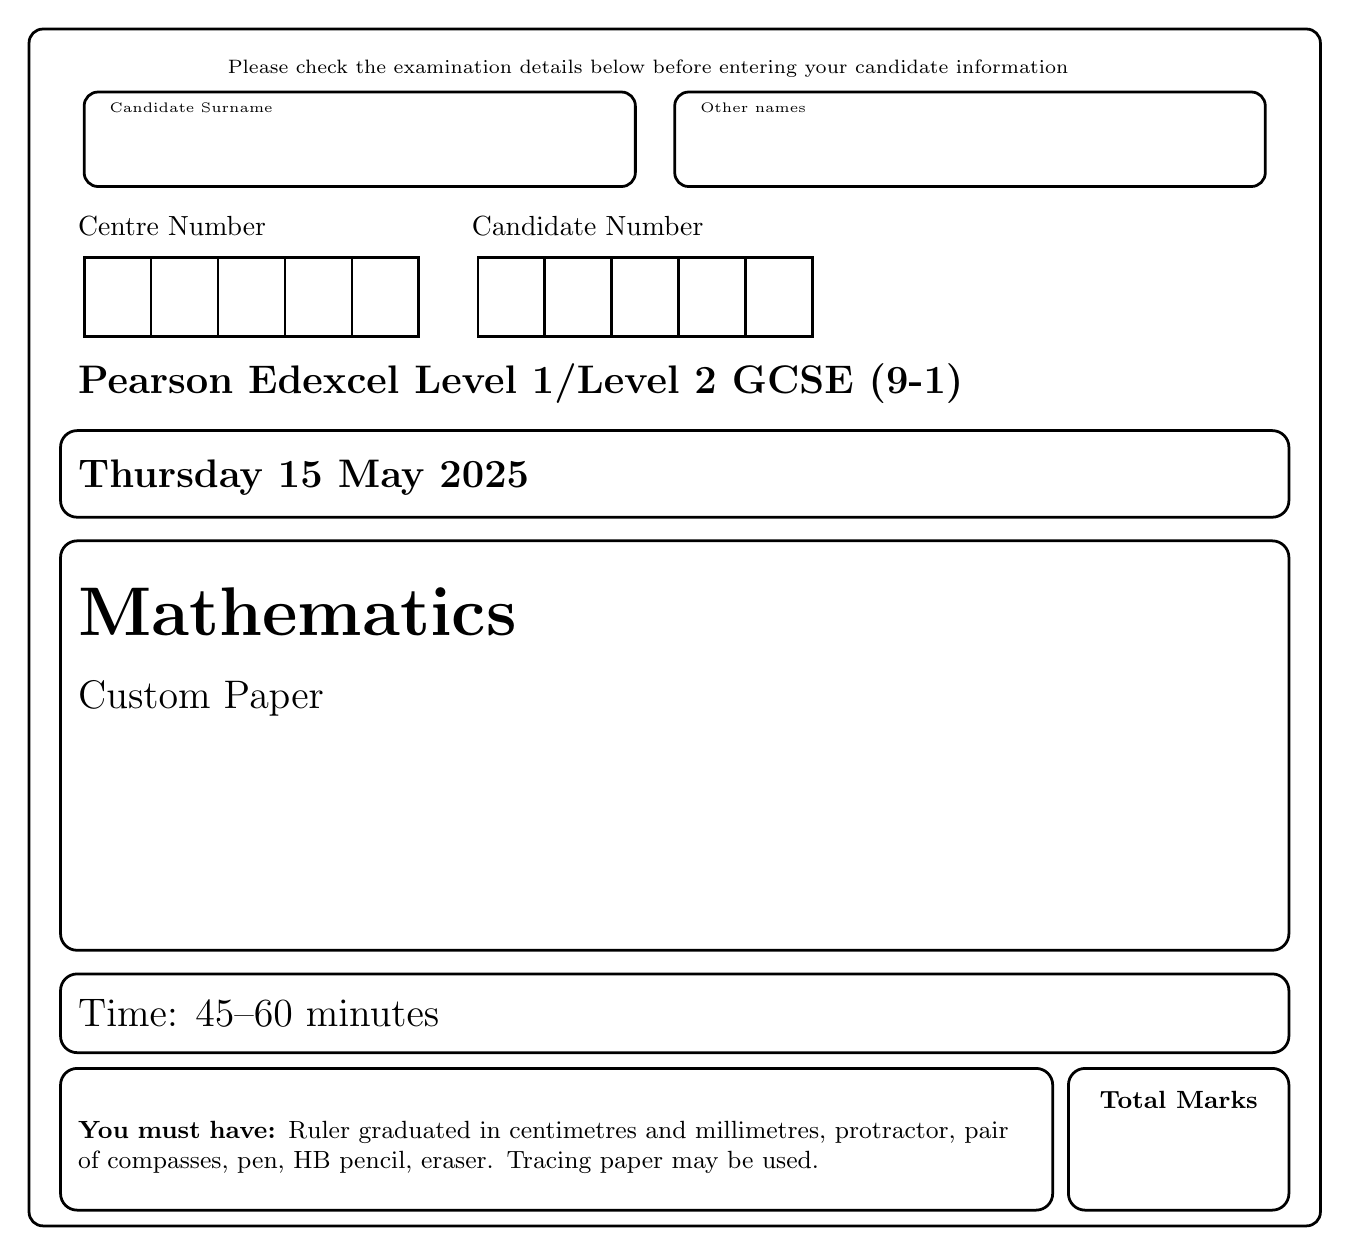
\begin{tikzpicture}[x=1cm,y=1cm]
% Outer main frame
  \draw[rounded corners=5pt, line width=1pt] (0.8,9.8) rectangle (17.2,25);

  % --------------------
  % Name section
  % --------------------

  % Surname & Other names boxes
  \node[anchor=west, font=\scriptsize] at (3.2,24.5) {Please check the examination details below before entering your candidate information};
  \draw[rounded corners=5pt, line width=1pt] (1.5,24.2) rectangle (8.5,23);
  \node[anchor=west, font=\tiny] at (1.7,24) {Candidate Surname};
  \draw[rounded corners=5pt, line width=1pt] (9.0,24.2) rectangle (16.5,23);
  \node[anchor=west, font=\tiny] at (9.2,24) {Other names};

  % Centre / Candidate labels
  \node[anchor=west] at (1.3,22.5) {Centre Number};
  \node[anchor=west] at (6.3,22.5) {Candidate Number};

  % Centre Number boxes (5 boxes)
  \foreach \i in {0,...,4} {
    \draw[line width=1pt] (1.5+\i*0.85,21.1) rectangle +(0.85,1);
  }
  % Candidate Number boxes (4 boxes)
  \foreach \i in {0,...,4} {
    \draw[line width=1pt] (6.5+\i*0.85,21.1) rectangle +(0.85,1);
  }

  % --------------------
  % Exam title lines
  % --------------------
  \node[font=\Large\bfseries, anchor=west] at (1.3,20.5) {Pearson Edexcel Level 1/Level 2 GCSE (9-1)};

  \draw[rounded corners=6pt, line width=1pt] (1.2,19.9)   rectangle (16.8,18.8);
  \node[font=\Large\bfseries, anchor=west] at (1.3,19.3) {Thursday 15 May 2025};

  % --------------------
  % Main exam box
  % --------------------
  \draw[rounded corners=6pt, line width=1pt] (1.2,13.3) rectangle (16.8,18.5);
  \node[font=\Huge\bfseries, anchor=west] at (1.3,17.6) {Mathematics};
  \node[font=\Large, anchor=west]  at (1.3,16.5) {Custom Paper};

  % --------------------
  % Time & Reference
  % --------------------
  \draw[rounded corners=6pt, line width=1pt] (1.2,12)   rectangle (16.8,13);
  \node[font=\Large, anchor=west] at (1.3,12.5) {Time: 45–60 minutes};
  

  % --------------------
  % Required items & Marks
  % --------------------
  \draw[rounded corners=6pt, line width=1pt] (1.2,10) rectangle (13.8,11.8);
  \node[font=\small, anchor=west, text width=12cm, align=left] at (1.3, 10.8) {\textbf{You must have:} Ruler graduated in centimetres and millimetres, protractor, pair of compasses, pen, HB pencil, eraser. Tracing paper may be used.};

  \draw[rounded corners=6pt, line width=1pt] (14,10) rectangle (16.8,11.8);
  \node[font=\small, anchor=center] at (15.4,11.4) {\textbf{Total Marks}};

\end{tikzpicture}
\end{center}

{\small
\begin{adjustwidth}{1.5cm}{1.5cm}

  {\large\bfseries Instructions\par}
  \begin{itemize}[%
      left=1em,
      label=\textbullet,
      topsep=0pt, 
      partopsep=0pt,
      parsep=0pt, 
      itemsep=0pt
    ]
    \item Use \textbf{black} ink or ball‐point pen.
    \item \textbf{Fill in the boxes} at the top of this page with your name, centre number and candidate number.
    \item Answer \textbf{all} questions.
    \item Answer the questions in the spaces provided\\
          \hspace*{1em}-- \textit{there may be more space than you need}.
    \item You must \textbf{show all your working}.
    \item Diagrams are \textbf{NOT} accurately drawn, unless otherwise indicated.
  \end{itemize}

  \vspace{0.5em}
  {\large\bfseries Information\par}
  \begin{itemize}[%
      left=1em,
      label=\textbullet,
      topsep=0pt, 
      partopsep=0pt,
      parsep=0pt, 
      itemsep=0pt
    ]
    \item The total mark for this paper is \textbf{@@TOTAL@@}
    \item The marks for \textbf{each} question are shown in brackets\\
          \hspace*{1em}-- \textit{use this as a guide as to how much time to spend on each question}.
  \end{itemize}

  \vspace{0.5em} 
  {\large\bfseries Advice\par}
  \begin{itemize}[%
      left=1em,
      label=\textbullet,
      topsep=0pt, 
      partopsep=0pt,
      parsep=0pt, 
      itemsep=0pt
    ]
    \item Read each question carefully before you start to answer it.
    \item Try to answer every question.
    \item Check your answers if you have time at the end.
  \end{itemize}
\end{adjustwidth}
}
}%


%PAGES_PLACEHOLDER

\vspace{1ex}

\hrule height 1pt

\vspace{1ex}

\hfill \textbf{TOTAL FOR PAPER IS @@TOTAL@@ MARKS}
\end{document}